%In diesem Unterkapitel sollten folgende Punkte behandelt werden:
%\begin{itemize}
%	\item	Was ist das Problem
%	\item 	Problemgeschichte?
%\end{itemize}
\section{Motivation}

In der Welt der Systeme mit Benutzerinteraktionen gibt es stets die Hürde, dass ``im Feld`` unvorhergesehene Probleme auftreten. Diese Systeme können bspw. Graphical User Interfaces (GUI) sein. Donald Norman \cite{TheProblemOfAutomation} argumentierte bereits 1989, dass bei komplexen Aufgaben und Umgebungen das Unerwartete erwartet werden muss. Nutzerfeedback ist notwendig um diese Situation aufzuklären und beheben zu können \cite{AnErrorReportingAndFeedbackComponent}.

In der Webentwicklung ist dieses Problem noch prägnanter, denn hier sind..
\begin{itemize}
	\item ..die Systeme selber meist um ein Vielfaches komplexer \cite{ManagingTheComplexityOfWebSystemsDevelopment},
	\item ..die Umgebungen komplex und unterschiedlich,
	\item ..die Nutzer meist weniger gut oder gar nicht geschult,
	\item ..die Nutzer eher unwissend, wie das System funktioniert \cite{AnErrorReportingAndFeedbackComponent} und
	\item ..die Nutzer stehen meist nicht im direkten Kontakt mit den Entwicklern \cite{EndUsersAsUnwittingSoftwareDevelopers}.
\end{itemize}

\begin{wrapfigure}[13]{r}{0.33\linewidth}
	\centering
	\vspace{-10pt}
	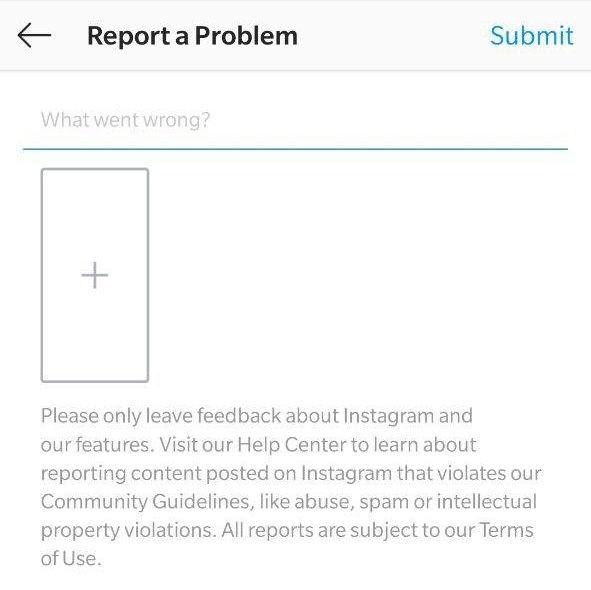
\includegraphics[width=\linewidth]{img/instagram-feedback/instagram-feedback.jpg}
	\caption{Formular aus der Instagram \cite{Instagram} Android App}
	\label{fig:instagram-feedback-example}
\end{wrapfigure}

\section{Problemstellung}

Aufgrund dieser Bedingungen werden bei Webprojekten Probleme im Feld erwartet. Zur Behebung dieser Mängel benötigen die Entwickler Informationen. Für Nutzer gibt es daher oftmals Formulare um diese Auffälligkeiten zu melden (Beispiel siehe rechts). Die Einbindung solcher Formulare ist zeit- und kostengünstig, kann aber nur erfolgreich sein, wenn die Nutzer verständliches und informatives Feedback geben können und wollen.

Bettenburg \etal \cite{WhatMakesAGoodBugReport} fanden bei Fehlerberichten eine Dissonanz zwischen dem was Entwickler als hilfreich empfanden und dem was Nutzer ihnen als Bericht lieferten. Eine besser zugeschnittene Lösung ist anzustreben. % \textbf{Wie kann den Entwicklern die Möglichkeit geboten werden, diese Probleme zu beheben?}

%\begin{itemize}
%	\item 	Was soll mit der Arbeit erreicht werden? Welche Ziele werden angestrebt?
%			Möglichst kurz und präzise geplante Ergebnisse umreißen. Daran werden
%			Ihre Resultate am Ende gemessen!
%\end{itemize}
\section{Zielsetzung}

Ziel dieser Arbeit ist es, zu erörtern, wie Fehler und Probleme, die ``im Feld`` auftreten, effektiv von Entwicklern und Betreibern identifiziert und behoben werden können. Entwickler und Betreiber sind die Hauptzielgruppe dieser Arbeit und werden nachfolgend \textbf{Stakeholder} genannt.

Im Zuge der Arbeit sollen folgende Fragen beantwortet werden:

\begin{enumerate}
	\item Was gibt es für Probleme bei Nutzern?
	\item Was sind häufige Problemursachen?
	\item Wie können diese Probleme identifiziert werden?
	\item Wie kann die Identifizierung mit einer Sofware vereinfacht werden?
	\begin{enumerate}
		\item Was ist der Aufwand?
		\begin{enumerate}
			\item bspw. Zeitaufwand bei der Integration von Software
		\end{enumerate}
		\item Was sind die Kosten für den Nutzer?
		\begin{enumerate}
			\item Wird die Leistung der Webapplikation beeinträchtigt?
			\item Werden persönliche Daten von ihm erhoben (Stichwort DSGVO)?
		\end{enumerate}
		\item Welche Probleme werden tatsächlich erkannt?
	\end{enumerate}
%	\item Was ist der aktuelle Stand der Technik? \\ 
%	Wenn es hier Ansätze gibt:
%	\begin{enumerate}
%		\item Welche Probleme werden hiermit behoben?
%		\item Was sind die Kosten für den Einsatz?
%		\item Was sind die Kosten für den Nutzer? (initiale Ladezeit, Datenlast)
%		\item Wie wird mit den Daten gehandhabt? (in Hinblick auf die DSGVO)
%	\end{enumerate}
\end{enumerate}

Am Ende der Arbeit soll dem Leser klar vermittelt worden sein, wie er diese Probleme identifiziert und ihnen nachhaltig begegnen kann. Risiken sowie Einschränkungen der Technologien und Methodiken sind dem Leser ebenso vermittelt worden.

\subsection{Abgrenzung}

Die zu erstellende Softwarelösung soll sich mit Webapplikationen beschäftigen, die dynamisch mit JavaScript erzeugt werden - auch Single-Page-Applications (SPAs) genannt. 

%\subsection{Abgrenzung}
%
%Diese Arbeit soll sich mit der GUI Entwicklung in der Webentwicklung beschäftigen. Weiterhin soll sich nicht auf den anfänglichen Entwicklungsprozess konzentriert werden, sondern auf bereits bestehende Software. Es soll keine benutzerorientierte Entwicklung \cite{UserCenteredWebDesign} beleuchtet oder angestrebt werden.

%\begin{itemize}
%	\item 	Wie wird vorgegangen, um das Ziel zu erreichen?
%	\item 	Warum ist die Arbeit so gegliedert, wie sie gegliedert ist?
%	\item 	Welche Aspekte werden nicht behandelt und warum?
%\end{itemize}
\section{Vorgehensweise}

Anfangs soll identifiziert werden, was alles für einen Nutzer ein Problem darstellen kann. Es muss sich bei den Problemen nicht nur um Laufzeitfehler o.Ä. handeln, sondern Logikfehler oder auch Verständnisprobleme führen zu einer Einschränkung der Nutzbarkeit. Hier soll eine Analyse aus der Literatur und ggf. einer Umfrage erstellt werden, um daraufhin grobe Problembilder zu klassifizieren.

Danach soll erörtert werden, welche Ursachen es für häufige Fehlerszenarien gibt. Darauf aufbauend könnten Aussagen getroffen werden, wie man diese bereits vorher vermeidet/reduziert.

Durch das gewonnene Verständnis über diese Probleme, soll nun ein Konzept erarbeitet werden. Dieses Konzept soll darauf abzielen zu den einzelnen Problembildern jeweils einen Ansatz zu finden, diese aufzuzeigen und den Stakeholdern Informationen zu liefern, die bei der Behebung notwendig sind (bspw. Geräteinformationen, Sitzungsinformationen, Logs, etc.).

Anhand des Konzeptes soll nun eine Softwarelösung entworfen werden. Hierbei soll es einerseits eine datenerhebende Komponente geben, welche mit in der Webapplikation läuft. Und andererseits soll es eine auswertende und informative Komponente geben, welche die Stakeholdern über die Probleme informiert und wichtige Informationen zur Behebung bereitstellt.

Nach dem Entwurf soll die Softwarelösung implementiert werden. Diese Implementierung soll zunächst projektunabhängig erfolgen.

Als letztes soll eine Webapplikation in der Open Knowledge GmbH hinzugezogen werden, in welche die Softwarelösung integriert werden soll. Nach der Integration sollen folgende Aspekte beleuchtet werden:

\begin{itemize}
	\item Wie einfach ist die Integration in ein bestehendes Projekt?
	\item Welche Problembilder können mit der Softwarelösung erkannt werden?
	\item Welchen Einfluss hat die Softwarelösung auf die Leistung? \\(Anhand von Aspekten wie Netzwerktraffic, Reaktionsgeschwindigkeit)
\end{itemize}

Als letztes soll ein Fazit über die Arbeit gezogen werden. Danach soll im Ausblick genannt werden, wie das Themengebiet und die erstellte Softwarelösung sich weiterentwickeln könnten.

% Da nun ein Basisverständnis gewonnen wurde, sollen etablierte Technologien wie Google Cloud \cite{GoogleCloudErrorReporting}, Dynatrace \cite{DynatraceDigitalExperienceMonitoring}, Sentry \cite{SentryForJavaScript} und LogRocket \cite{LogRocket} näher betrachtet werden. Durch die Erörterung des Stands der Technik sollen folgend Empfehlungen ausgesprochen werden, für welche Projekte welche Technologie oder Kombination von Technologien sinnvoll ist. Sollte keine Technologie als angemessen betrachtet werden, so soll basierend auf den Anforderungen ein Vorschlag gemacht werden, wie so eine Technologie aussehen könnte.
